\chapter{Data and analysis}

The full description of the survey is in: D. J. Sand et. al. \citeyear{Reference11}

MegaCam wide field imager on the CFHT (Canada-France-Hawii Telescope). The cluster sample consisted of 101 clusters within the range of redshifts from 0.05 < z< 0.55

58 clusters from the MENEACs (Multi-Epoch Nearby Cluster Survey)

The meneacs clusters represent all clusters in the BAX X-ray cluster database that are observable for the CFHT (Canada France Hawaii Telescope)

About 60 clusters, but we used only 30 for the final studies and paid special attention to 10, marked with *

G, U, I and R images

\begin{table}[]
\centering

\begin{tabular}{ccccc}
Cluster & $z$   & $\sigma(km/s)$ & $d(Mpc)$ & $\theta_{E}(")$ \\ \hline \hline
A1033   & 0.126 & 762            & 540 & 14.6155  \\
A1068*  & 0.138 & 740            & 591.4 & 13.5945  \\
A1132   & 0.136 & 727            & 582.9 & 13.1515   \\
A119*   & 0.044 & 875            & 188.6 & 21.0798   \\
A1413*  & 0.143 & 881            & 612.9 & 19.1569   \\
A1650   & 0.084 & 720            & 360 & 13.6758   \\
A1651   & 0.085 & 903            & 364.3 & 21.4876   \\
A1795   & 0.062 & 778            & 265.7 & 16.3514   \\
A2029*  & 0.077 & 1152           & 330 & 35.2776   \\
A2050   & 0.118 & 854            & 505.7 & 18.5258   \\
A2055   & 0.102 & 697            & 437.1 & 12.5642   \\
A2064   & 0.108 & 675            & 462.9 & 11.7048   \\
A2065*  & 0.073 & 1095           & 312.9 & 32.0110   \\
A2069   & 0.116 & 966            & 497.1 & 23.7574   \\
A2142*  & 0.091 & 1086           & 390 & 30.8756   \\
A2319*  & 0.056 & 1101           & 240 & 32.9563   \\
A2420   & 0.085 & ~800           & 364.3 & 16.8653   \\
A2440   & 0.091 & 766            & 390 & 15.3608   \\
A2597   & 0.085 & 682            & 364.3 & 12.2569   \\
A2627   & 0.126 & ~800           & 540 & 16.1096   \\
A2703   & 0.114 & ~800           & 488.6 & 16.3307   \\
A399    & 0.072 & ~800           & 308.6 & 17.1049   \\
A553    & 0.066 & ~800           & 282.9 & 17.2155   \\
A655*   & 0.127 & ~800           & 544.3 & 16.0911   \\
A754*   & 0.054 & ~800           & 231.4 & 17.4367   \\
A763    & 0.085 & ~800           & 364.3 & 16.8653   \\
A795    & 0.136 & ~800           & 582.9 & 15.9252   \\
A85*    & 0.055 & ~800           & 235.7 & 17.4182   \\
A961    & 0.124 & ~800           & 531.4 & 16.1464   \\
A990    & 0.144 & ~800           & 617.1 & 15.7778   
\end{tabular}
\caption[Abell Clusters and their redshift]{Abell clusters and their redshifts as given by C. Bildfell et. al. \citeyear{Reference6}. Marked with * the chosen clusters with the most promising features}
\end{table}

The original images have dimensions of [11000:11000] pixels but since our relevant region is the center of the cluster where the BCG is located, we cut the images with dimension of [1000,1000] for the color analysis and [4000:4000] to characterize the colors and discriminate between cluster and non-cluster members.

The INT images were obtained using multiple exposures so it was necessary to make a mosaic of them using SWARP.

\section{Stellar populations}
 
Galaxy clusters contain a population of stars gravitationally unbound to individual galaxies, yet still bound to the clusters overall gravitational potential, created by the stripping of stars from galaxies during interactions and mergers

\section{Stellar Populations}

Mass-to-light ratios of early-type galaxies are of particular interest to understand the tilt of the fundamental plane. Virial relations imply that the effective surface brightness $I_{\text{eff}}$, the effective radius $r_{\text{eff}}$ and the central velocity dispersion $\sigma_{0}$ in hot stellar systems are not independent of each other. This is revealed by the fundamental plane of early type galaxies.

The Salpeter IMF implies more low-mass stars and a higher mass-to-light ratio. In the R-band the scaling between the two cases is $\Upsilon_{\text{Salp}}\approx 1.56\Upsilon_{\text{Krou}}$

A Koupra IMF finds a value of around 4 for the mass to light ratio $\Upsilon$. (R. J. Smith \citeyear{Reference5}). Massive galaxies - Salpeter is a good IMF. Salpeter is heavier than Kroupa. Salpeter mass function is $n(\textrm{M})\propto \textrm{M}^{-2.3}$ 

Large M/L ratios could arise either from an excess of faint dwarf stars in a ``bottom heavy" IMF, or from an excess of dark remnants in a ``top heavy" IMF" (Russell J. Smith and John R. Lucey \citeyear{Reference7}).

\section{IMF in BCGs}

Several recent studies have investigated whether the IMF systematically varies with galaxy mass, in particular among elliptical galaxies. These analyses are mostly based on two independent approaches. The first is an indirect method, where galaxy stellar masses are determined from stellar population synthesis models that actually do not resolve the IMF: the IMF is adjusted until the population-synthesis mass-to-light ratio matches independent constraints from dynamics and/or lensing. The second, direct method uses features in galaxy spectra that are particularly sensitive to the presence of, e.g., dwarf stars to determine the IMF directly from spectroscopic observations. Both approaches come to the same result: although there is significant galaxy to galaxy scatter, lower mass early-type galaxies (with dispersions $\sigma \approx 200$km/s) seem to be roughly consistent with a Milky-Way type IMF (e.g. a Kroupa or Chabrier IMF). In high-dispersion elliptical galaxies, however, stellar mass-to-light ratios are about a factor of 2 times higher than expected from a Kroupa IMF. Direct studies specifically indicate that the IMF in massive galaxies seems to be more dwarf dominated than in the Milky-Way (and can be described, e.g., by a Salpeter IMF).

\textbf{Van der Vurg Thesis:} \textit{The adopted $\text{M}_{\star}/L$ is a major systematic uncertainty in any study and depends on the assumed IMF due to differences in the contribution of low mass stars to the total mass. We transform the results from other studies to the Chabrier IMF by subtracting 0.24 dex in mass for a Salpeter IMF, or adding 0.04 dex to the mass for a Kroupa IMF. The $\text{M}_{\star}/L$ depends on galaxy type, but due to the lack of multi-wavelength photometry, it is often assumed that all cluster galaxies are composed of the same stellar population. If one assumes an old stellar population (and therefore a high $\text{M}_{\star}/L$), the mass of the late-type galaxies (and thus the cluster as a whole) is over-estimated.} \citeyear{Reference2}

%this image is commented because it's not too relevant for our purposes
\begin{comment}
\begin{figure}[H]
\centering
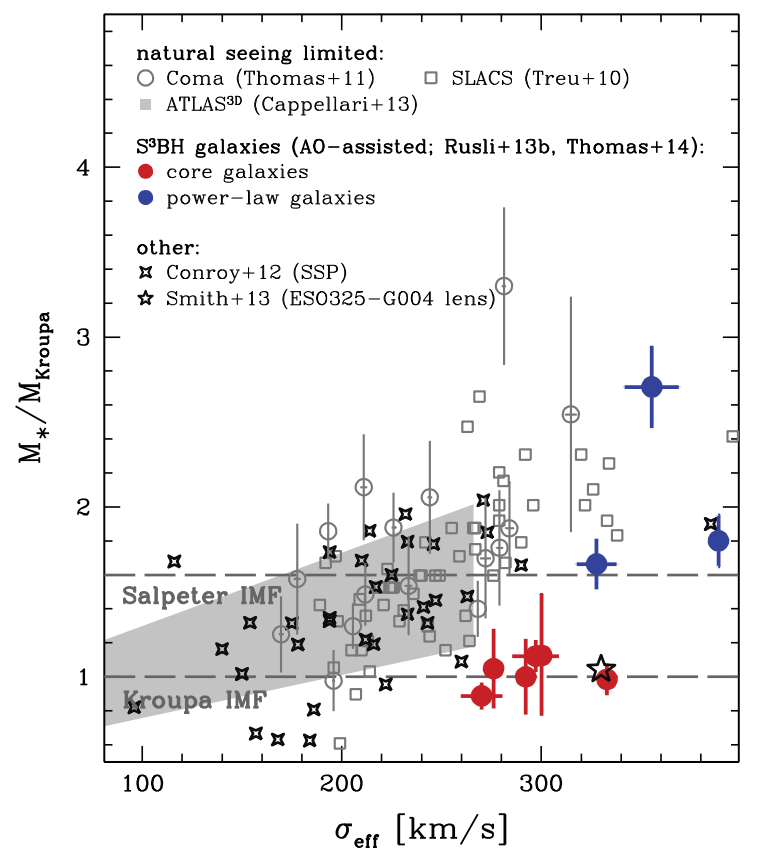
\includegraphics[width=12cm]{images/IMFs.png}
\caption[R]{R}
\end{figure}
\end{comment}

number of stars per unit mass

Kroupa, Chabrier, Salpeter, 

%this image is commented because it's not too relevant for our purposes
\begin{comment}
\begin{figure}[H]
\centering
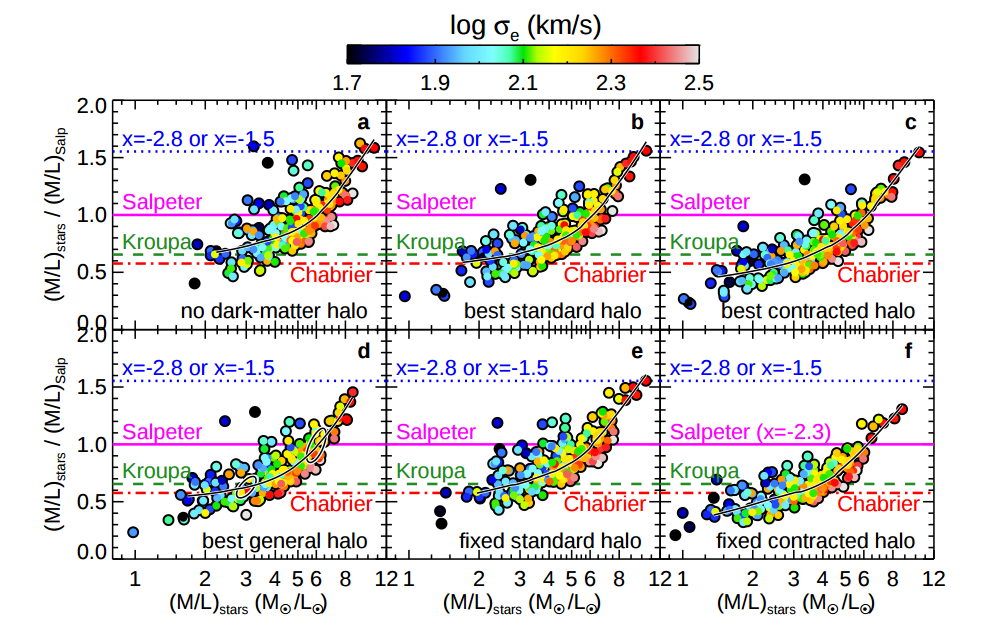
\includegraphics[width=12cm]{images/IMFs_paper.png}
\caption[The systematic variation of the IMF in early-type galaxies.]{The systematic variation of the IMF in early-type galaxies, Cappellari et. al. \citeyear{Reference19}.}
\end{figure}
\end{comment}

Heavyweight

It's difficult to see how much of the faint stars contribute to the mass of the system. We only see the new bright ones

For stars, measurements of the luminosity function can be used to derive the Initial Mass Function (IMF). For galaxies, this is more difficult because Mass to light ratio (M/L) of the stellar population depends upon the star formation history of the galaxy. Bulges have heavier IMFs than disks

Several recent studies have presented evidence for ``heavyweight" IMFs in giant ellipticals, with a mass-to-light-ratio twice that of a Milky Way like IMF. 


\section{Sextractor}

Segmentation image that will be used as a mask image (bad pixels) for \texttt{GALFIT}

We need to discriminate between field stars and the galaxies of the cluster so in order to do this, we used some of the parameters found by \texttt{SEXTRACTOR} that allow us to constraint the fitted data. These are class-star, flux\_radius, and FWHM (full wicth half maximum). Class-star uses the neural network star/galaxy of \texttt{SEXTRACTOR} that will give values close to 1 for stars and 0 for galaxies. flux\_radius, and FWHM are closely related to each other and give the radius which contains half of the light of the object so it will be small for stars and bigger for extended objects.

In order to extract the same objects and make the segmentation masks for the desired objects in the different filters, we used \texttt{SEXTRACTOR} on dual mode

Color magnitude diagram for A1068

we used a zero point magnitude of 30

\begin{figure}[H]
\centering
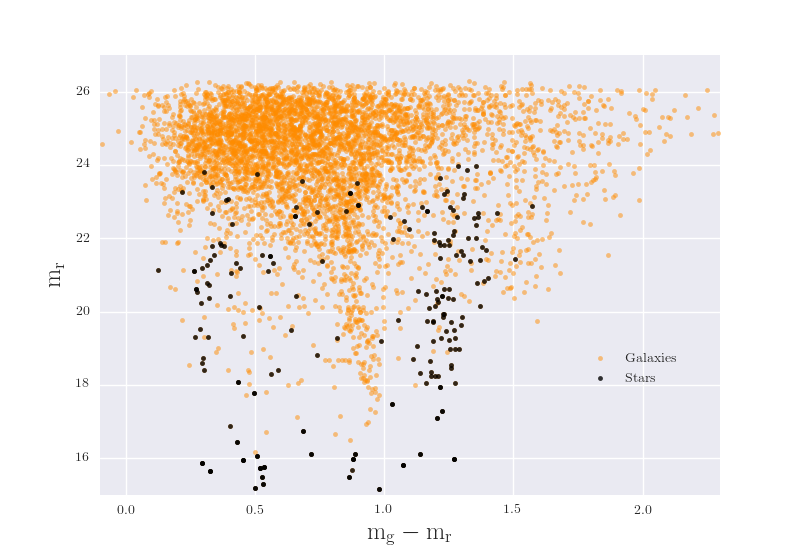
\includegraphics[width=12cm]{images/color_mag.png}
\caption[Color Magnitude diagram of A1068]{Color Magnitude diagram of A1068 with the differentiation of stars from galaxies}
\end{figure}

Mag vs flux rad to discriminate

\begin{figure}[H]
\centering
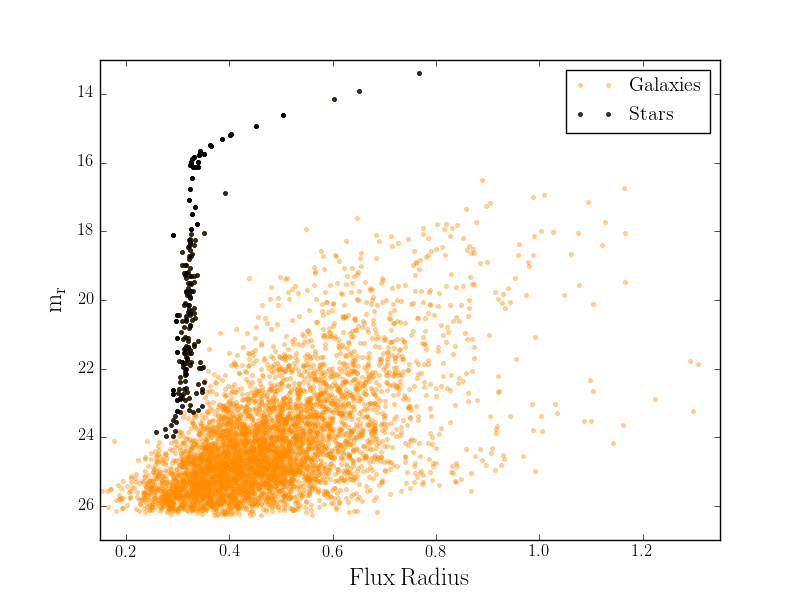
\includegraphics[width=12cm]{images/mag_vs_flux_rad.png}
\caption[Magnitude vs Flux radius of A1068]{Magnitude vs Flux radius of A1068 to identify the galaxies using the criteria of their flux distribution}
\end{figure}

\section{Galfit}

\texttt{GALFIT} (Peng et. al \citeyear{Reference20}) fits two dimensional profiles so it is a useful tool to remove the light from the BCG and allow us to observe background objects

Fit Sersic profiles with n=4 which is de Vaucouleurs profile. 

A first run gives us a rough idea of the true position of the center of the BCG so we can set this values in a second run for each cluster. We needed to combine different Sersic parameters, as well as Fourier and bending modes for some of the BCGs.

We use the segmentation masks given by \texttt{SEXTRACTOR} to mask bright objects in the fitting of the BCG

the fitting of many objects (not only the BCG)

the best results were given when we masked the innermost region of the BCG so the fitting will put more weight in the rest of the profile, thus reducing most of the light that hides the background objects.

we have to take into account the magnification bias

The parameters C0, B1, B2, F1, F2, etc. listed below are hidden from the user unless he/she explicitly requests them.  These can  be tagged on to the end of any previous components except, of course, the PSF and the sky -- although \texttt{GALFIT} won't bar you from doing so, and will just ignore them.  Note that a Fourier or Bending mode amplitude of exactly 0 will cause \texttt{GALFIT} to crash because the derivative image \texttt{GALFIT} computes internally will be entirely 0.  If a Fourier or Bending amplitude is set to 0 initially \texttt{GALFIT} will reset it to a value of 0.01.  To prevent \texttt{GALFIT} from doing so, one can set it to any 
other value.

Bending modes
B1)  0.07      1        Bending mode 1 (shear)
B2)  0.01      1        Bending mode 2 (banana shape)
B3)  0.03      1        Bending mode 3 (S-shape)

Azimuthal fourier modes
F1)  0.07  30.1  1  1   Az. Fourier mode 1, amplitude and phase angle
F2)  0.01  10.5  1  1   Az. Fourier mode 2, amplitude and phase angle
F6)  0.03  10.5  1  1  Az. Fourier mode 6, amplitude and phase angle
F10)  0.08  20.5  1  1   Az. Fourier mode 10, amplitude and phase angle
F20)  0.01  23.5  1  1   Az. Fourier mode 20, amplitude and phase angle

Traditional Diskyness/Boxyness parameter c
C0) 0.1         0       traditional diskyness(-)/boxyness(+)

The masks:

\begin{figure}[H]
\centering
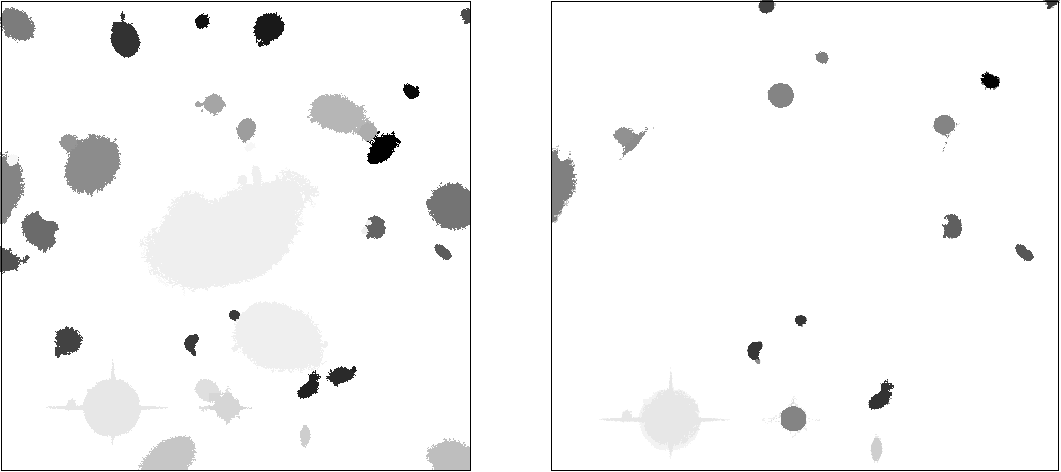
\includegraphics[width=15cm]{images/masks.png}
\caption[Segmentation images]{Segmentation images produced by \texttt{SEXTRACTOR} and used as mask files for the galfit extraction. Left panel is the original mask with all the bright objects. Right panel is the mask after the substraction of the regions surrounding the cluster galaxies to be fitted with \texttt{GALFIT}.}
\end{figure}

The colors are inverted for an easier visualization of the image. The fainter regions are actually the most luminous objects because \texttt{GALFIT} assigns increasing numbers starting from the brightest one, that is the BCG in this case

The original image, the fitted models and the output are presented here:

\begin{figure}[H]
\centering
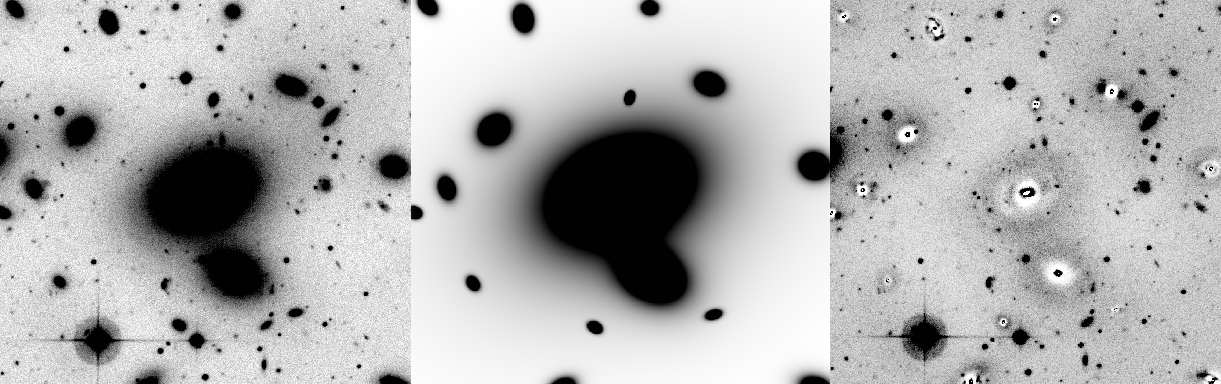
\includegraphics[width=15cm]{images/galfit.png}
\caption[Galfit results]{Galfit procedures. Left: Original image in zscale with the clear BCG expanding across a significant region of the central area. Middle: The models fitted by \texttt{GALFIT} for all the selected cluster galaxies. Right: Residual image after the substraction of the model galaxies.}
\end{figure}

\section{Color images} 

We use IRAF to make the color images using our g,r,u,i bands. Let's use ABELL754 which is a low redshift galaxy cluster with a calculated mass of $\text{M}_{200}=9.8\times 10^{15} \text{M}_{\odot}$ (Sifon et. al. \citeyear{Reference9})

Here we take an isothermal sphere to model the Einstein ring in a distance of background objects of z=1

We made a color image of the original center of the cluster without subtracting the BCG in order to differentiate between cluster members from background galaxies and field stars. This allows us to fit only the cluster galaxies. 

\begin{figure}[H]
\centering
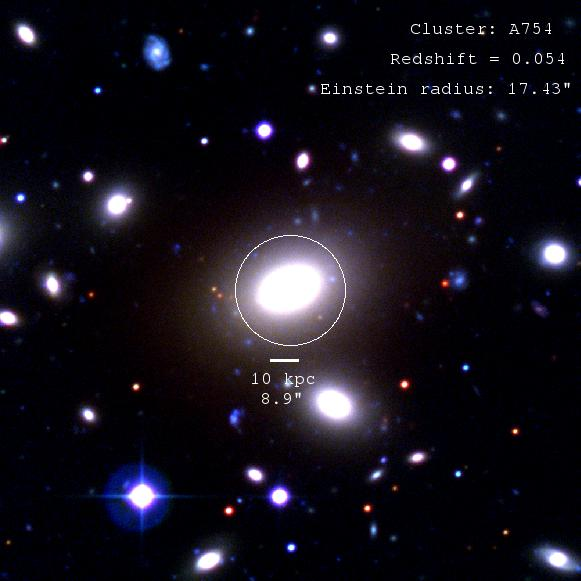
\includegraphics[width=12cm]{images/cA754.jpg}
\caption[Color image of A754]{Color image of A754 cluster (filters i,g,u) with its Einstein radius calculated for an isothermal sphere of a background object at $z=1$.}
\end{figure}

After choosing the galaxies that belong to the cluster by comparing their relative colors, we subtracted them using \texttt{GALFIT} and made the color image again changing the scaling values with the task \texttt{CONVERT} of \texttt{IRAF} so that we see can see the color contrast to search for good candidates of lensed objects. By looking at this reduced color image, we have another visual constraint to choose the clusters in which it would be worth to do photometric redshifts and search for objects with the same redshift in different locations around the very center of the BCG (object that has suffered strong lensing). 

\begin{figure}[H]
\centering
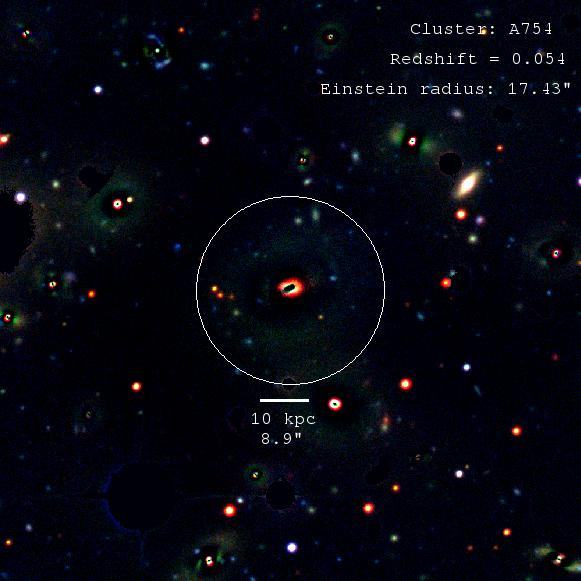
\includegraphics[width=12cm]{images/cA754_galfit.jpg}
\caption[Color image of A754 after fitting the bright objects]{Color image of A754 cluster (filters i,g,u) after the substraction of the bright cluster galaxies.}
\end{figure}

Because we have 4 bands we were able to make different color images to see the contrast and make combinations that would allow us to see better the very red and very blue objects, in the following figure we have the g-r, i-r-g and i-g-u color images for three clusters. 

\begin{figure}[H]
\centering
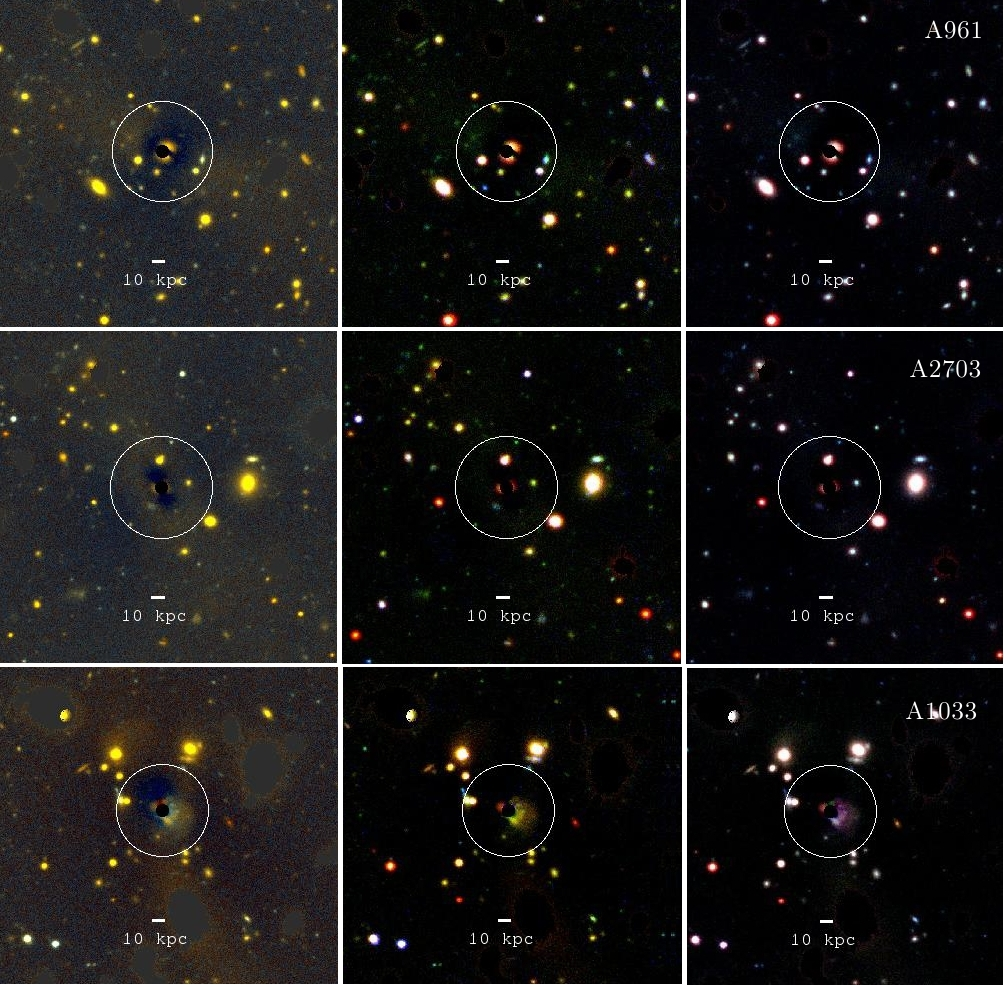
\includegraphics[width=15cm]{images/full_small.jpg}
\caption[Color images for various clusters]{Different color images for different combination of the g,r,u,i filters for the clusters A961, A2703, A1033. Left column for the images constructed only with the g and r filter, central column for i,g,r and right column for i,g,u.}
\end{figure}

\section{Photometric Redshifts}

We use the \textit{COSMOS2015} (Laigle et. al \citeyear{Reference21}.) catalogue that contains photometric redshift of over half million galaxies in multiple bands to put another constraint in our study.

We use the matched catalogue for CFHT by Remco Van der Burg and use the r-band. Our limiting magnitude is 23 in that band so we estimate the number of galaxies per redshift bin that we would expect to see in our sample with that limiting magnitude.

This sets an interesting constraint on what to expect in the inner region of the BCG and give us more information about where to search for good candidates.

The limiting magnitude is found using \texttt{SEXTRACTOR} that gives a good confidence on the detection of objects.

The COSMOS catalogue contains one square arcmin so we use this result to see what order  we should spect from background objects.

To measure the photometric redshift of the galaxies (after filtering out the stars) in the inner region of the cluster after the subtraction of the BCG, we use the photometric redshift code EAZY (Brammer et. al 2008) which uses an extensive collection of spectral energy distributions for galaxies in the range $0<z<4$. Fortunately, the code includes library from CFHT in the I and U bands but doesn't have the filters in the G and R bands so I used the SUBARU survey filter information to be able to compute the photometric redshifts using four bands.

citation of EAZY ``Brammer, van Dokkum and Coppi, \citeyear{Reference22}" 
